% KansasLava-AK.tex
\begin{hcarentry}{Web Technologies}
\label{kuwebtech}
\report{Andrew Farmer and Andy Gill}% if this needs one name, use Andrew Farmer
\participants{Andrew Farmer, Andy Gill}
\status{ongoing}
\makeheader

At KU, we are interested in providing better support for
interactive applications in Haskell by building on top of existing web technologies,
like the fast Chrome browser, HTML5, and JavaScript. This is motivated
partly by having easy tools to interactively teach programming in Haskell,
and partly by the needs of the HERMIT\cref{HERMIT} project.

Towards this, we have developed a lightweight web framework called {\tt Scotty}.
Modeled after Ruby's popular Sinatra framework, Scotty is intended to
be a cheap and cheerful way to write RESTful, declarative web applications.
Scotty borrows heavily from the Yesod \cref{Yesod} ecosystem, conforming
to the WAI \cref{WAI} interface and using the fast Warp \cref{Warp} web server
by default. More information can be found at the link below.

On top of {\tt Scotty}, we have built a simple interface
into the HTML5 Canvas mechanism, called {\tt blank-canvas}.
This was constructed primarily as a teaching tool and
a proof-of-concept design. Here is an example of
a teaching application which prints squares to the canvas,
based on where the user clicks the mouse.

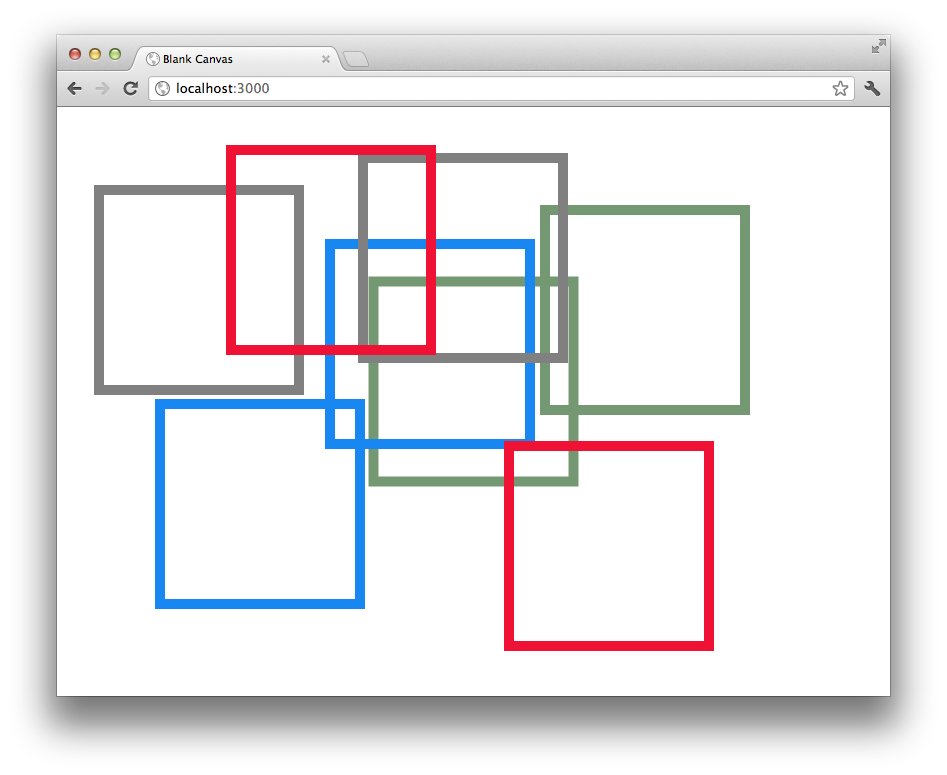
\includegraphics[width=0.47\textwidth]{html/squares.png}

Simple interactive games can be developed using this API,
and new Haskell programmers found it straightforward to use.
Unbeknown to us, {\tt blank-canvas} was also used in a high-school
level functional programming class being lead by Alwyn Goodloe.

We are now working to generalize the ideas in {\tt blank-canvas} by
creating a framework to handle arbitrary asynchronous Javascript events
and DOM manipulation via a server-side Haskell DSL. This DSL will make it possible to control
a browser-based UI using well known Haskell patterns, such as Functional
Reactive Programming.

All package are available from hackage, or will be shortly.

\FurtherReading
\begin{compactitem}
  \item \url{http://www.ittc.ku.edu/csdl/fpg/Tools/Scotty}
  \item \url{http://www.ittc.ku.edu/csdl/fpg/Tools/BlankCanvas}
\end{compactitem}

\end{hcarentry}
